\documentclass[man, noextraspace, floatsintext]{apa6}\usepackage[]{graphicx}\usepackage[]{color}
%% maxwidth is the original width if it is less than linewidth
%% otherwise use linewidth (to make sure the graphics do not exceed the margin)
\makeatletter
\def\maxwidth{ %
  \ifdim\Gin@nat@width>\linewidth
    \linewidth
  \else
    \Gin@nat@width
  \fi
}
\makeatother

\definecolor{fgcolor}{rgb}{0.345, 0.345, 0.345}
\newcommand{\hlnum}[1]{\textcolor[rgb]{0.686,0.059,0.569}{#1}}%
\newcommand{\hlstr}[1]{\textcolor[rgb]{0.192,0.494,0.8}{#1}}%
\newcommand{\hlcom}[1]{\textcolor[rgb]{0.678,0.584,0.686}{\textit{#1}}}%
\newcommand{\hlopt}[1]{\textcolor[rgb]{0,0,0}{#1}}%
\newcommand{\hlstd}[1]{\textcolor[rgb]{0.345,0.345,0.345}{#1}}%
\newcommand{\hlkwa}[1]{\textcolor[rgb]{0.161,0.373,0.58}{\textbf{#1}}}%
\newcommand{\hlkwb}[1]{\textcolor[rgb]{0.69,0.353,0.396}{#1}}%
\newcommand{\hlkwc}[1]{\textcolor[rgb]{0.333,0.667,0.333}{#1}}%
\newcommand{\hlkwd}[1]{\textcolor[rgb]{0.737,0.353,0.396}{\textbf{#1}}}%

\usepackage{framed}
\makeatletter
\newenvironment{kframe}{%
 \def\at@end@of@kframe{}%
 \ifinner\ifhmode%
  \def\at@end@of@kframe{\end{minipage}}%
  \begin{minipage}{\columnwidth}%
 \fi\fi%
 \def\FrameCommand##1{\hskip\@totalleftmargin \hskip-\fboxsep
 \colorbox{shadecolor}{##1}\hskip-\fboxsep
     % There is no \\@totalrightmargin, so:
     \hskip-\linewidth \hskip-\@totalleftmargin \hskip\columnwidth}%
 \MakeFramed {\advance\hsize-\width
   \@totalleftmargin\z@ \linewidth\hsize
   \@setminipage}}%
 {\par\unskip\endMakeFramed%
 \at@end@of@kframe}
\makeatother

\definecolor{shadecolor}{rgb}{.97, .97, .97}
\definecolor{messagecolor}{rgb}{0, 0, 0}
\definecolor{warningcolor}{rgb}{1, 0, 1}
\definecolor{errorcolor}{rgb}{1, 0, 0}
\newenvironment{knitrout}{}{} % an empty environment to be redefined in TeX

\usepackage{alltt}
\newcommand{\bibfile}{C:/Users/jep2963/Documents/Bibliography/Behavioral_observation-APP}  

\usepackage[natbibapa]{apacite}
\newcommand{\citetal}[1]{\shortcites{#1}\citet{#1}}

\raggedbottom

\usepackage{amssymb}
\usepackage{amsmath}
\usepackage{amsthm}
\newtheorem{lemma}{Lemma}

\usepackage{graphicx}

\usepackage{fixltx2e}
\usepackage{subcaption}
\usepackage{float}

\usepackage{array}
\usepackage{multirow}
\usepackage{rotating}
\setlength{\rotFPtop}{0pt plus 1fil}
\usepackage[draft]{changes}

\geometry{twoside=false, top=1in, bottom=1in, left=1in, right=1.2in}
\usepackage[textwidth=1in, textsize=tiny]{todonotes}

\newcommand{\Prob}{\text{Pr}}
\newcommand{\E}{\text{E}}
\newcommand{\Cov}{\text{Cov}}
\newcommand{\corr}{\text{corr}}
\newcommand{\Var}{\text{Var}}
\newcommand{\iid}{\stackrel{\text{iid}}{\sim}}
\newcommand{\logit}{\text{logit}}
\newcommand{\cll}{\text{cll}}


\title{Estimating the prevalence and incidence of a state behavior: Models for interval recording data and novel observation systems}
\shorttitle{ESTIMATING PARAMETERS OF A STATE BEHAVIOR}
\author{James E. Pustejovsky and Daniel M. Swan}
\leftheader{Pustejovsky & Swan}
\affiliation{The University of Texas at Austin}
 
\abstract{Data based on direct observation of behavior are used widely in many areas of educational and psychological research, particularly in applied research areas such as the treatment of behavioral disorders. 
A number of different methods are used to code or record data from direct observation, including continuous recording, momentary time sampling (MTS), partial interval recording (PIR, also known as one-zero sampling, modified frequency sampling, Hansen sampling, or simply time-sampling), and whole interval recording (WIR). 
Among these methods, PIR and WIR have long been recognized as problematic because, as typically reported, the mean of such data measures neither the prevalence nor the incidence of a behavior. 
Though the problems with these methods have long been recognized, little research has examined methods of analyzing interval recording data other than simply taking the mean. 
This paper proposes a Alternating Poisson Process model for interval recording data that permits estimation of both prevalence and incidence via maximum likelihood or penalized maximum likelihood methods. 
The paper also describes some novel observation recording methods that involve combinations of MTS, PIR, and WIR, and that offer considerably more efficient estimators of prevalence and incidence.}

\keywords{behavioral observation; interval recording; alternating Poisson process; Markov chain}

\authornote{James E. Pustejovsky, Department of Educational Psychology, University of Texas at Austin. Daniel M. Swan, Department of Educational Psychology, University of Texas at Austin.

Address correspondence to James E. Pustejovsky, Department of Educational Psychology, University of Texas at Austin, 1 University Station D5800, Austin, TX 78712. Email: pusto@austin.utexas.edu.}
\IfFileExists{upquote.sty}{\usepackage{upquote}}{}
\begin{document}


\maketitle

Measurements derived from systematic, direct observation of human behavior are used in many areas of psychological and educational research. 
For example, direct observation of student classroom behavior is a primary component of several existing instruments for screening and diagnosis of emotional and behavioral problems \citep{Volpe2005observing}; direct observation of childrens' challenging behavior in home settings has been employed to collect pre- and post-test measures in randomized trials of behavioral interventions \citep[e.g.,][]{Durand2012positive}; and direct observation of infant-parent interaction patterns is employed in studies of child development \citep{Mann1991time} and cross-cultural differences \citep{Bornstein2002measurement}. 
Direct observation also plays a prominent role in single-case research, where it is used to measure changes in behavior over time and assess individual responses to intervention \citep{Kazdin2011single}.

Systematic direct observation procedures require that the behavior of interest have a clear operational definition, so that its occurrence or absence can be judged at a given point in time. 
In forming such an operationally definition, is useful to distinguish between behaviors that are \textit{events}, where each occurrence is of negligible duration, versus behaviors that are \textit{states}, where individual episodes of behavior have positive duration \citep{Altmann1974observational}. 
The primary characteristic of an event behavior is its incidence, or frequency of occurrence per time unit. 
In contrast, a state behavior has two primary characteristics: incidence (the frequency with which new episodes of the behavior begin, per time unit) and prevalence, or the proportion of time that the behavior occurs. Given an operationally defined behavior, measurements of its characteristics are obtained by observing the behavior (either in person, or by video-recording) for a specified length of time. 
The pattern of behavioral episodes over the course of an observation session--that is, what a human observer actually perceives--is often called the \textit{behavior stream}. 

There are several different procedures for recording data during direct observation, varying in ease of implementation, the level of detail in the resulting data, and the aspect of behavior to which the resulting measurement corresponds \citep[for surveys of major recording procedures, see][]{Altmann1974observational, Ayres2010dependent, Hartmann1990observational, Primavera1996measurement}. 
The most intensive procedure is continuous recording (sometimes called duration recording or real-time recording), in which the observer records the time at which each event begins and ends.
Data from continuous recording is very rich, in that it permits direct estimation of prevalence, incidence, and other aspects of the behavior stream; it can also be subjected to more sophisticated forms of modeling \citep[e.g.,][]{Bakeman2011sequential, Haccou1992statistical}. 
However, less effort-intensive data collection methods are often required, particularly for use in clinical and applied research settings. 

Other commonly used systems for collecting behavioral data do not capture a complete record of the behavior during an observation session, but rather involve making observations only intermittently. 
Among intermittent recording systems, the three main procedures are momentary time sampling, partial interval recording, and whole interval recording. 
In all three methods, an observation session is divided into a fixed number of equally spaced intervals, of perhaps 10 or 15 s in length, and a binary data-point is recorded for each interval. 
The systems differ only in the rule for scoring each interval. 
Using momentary time sampling (MTS), an interval is scored as a one if a behavioral event is happening during the final moment of the interval (and is otherwise scored as a zero). 
Using partial interval recording (PIR), an interval is scored as a one if the behavior occurs at any point during the interval. 
Using whole interval recording (WIR), an interval is scored as a one only if the behavior occurs for the entire duration of the interval. 
In some PIR and WIR systems, a small length of time is left between each interval so that the observer does not have to maintain continuous attention. 

In many applications, the interval-by-interval data generated by these recording systems is summarized by the proportion of intervals scored as a one. 
Often, only this summary proportion is used for later analysis, where it is interpretted as a measure of prevalence. 
However, the circumstances under which it is reasonable to reduce the data to a summary proportion depends on the recording system used to collect the data. 

Under quite general modeling assumptions, the proportion of MTS intervals is an unbiased estimate of prevalence \citep{Rogosa1991statistical}. 
Thus, reducing the data to the summary proportion may be quite reasonable if the investigator's interest is solely in the prevalence of the behavior. 
However, simple summaries of MTS data do not provide a clear measure of the behavior's incidence. 
Even if not of substantive interest, estimates of incidence are  are necessary for assessing the magnitude of measurement error in the prevalence estimates. 

\citet{Brown1977estimation} described a method for estimating both prevalence and incidence from MTS data. 
Their approach was to first posit a stochastic process for the underlying stream of behavior, as perceived by the observer, and then to consider the implications of observing the process intermittently via an MTS system. 
The particular model they considered was an Alternating Poisson Process, which is a simple, two-state continuous time Markov chain where transitions between states follow exponential distributions. 
The Alternating Poisson Process implies that interval-by-interval MTS scores follow a discrete-time Markov chain. 
Under the model, \citet[see also \citealp{Griffin1983parametric}]{Brown1977estimation} provided closed-form expressions for the maximum likelihood estimators of prevalence and incidence and the associated asymptotic covariance matrix.

Unlike MTS, PIR and WIR systems do not produce clearly interpretable summary measurements. 
Rather, the PIR summary proportion systematically over-estimates prevalence and the WIR summary proportion systematically under-estimates prevalence; in both cases, the extent of the bias depends on the incidence of the behavior as well as operational features of the recording system \citep{Kraemer1979one, Rogosa1991statistical}, making the construct interpretation of such data quite difficult. 
Consequently, methodologists have long argued against the use of PIR and WIR systems \citep[cf.]{Altmann1974observational, Mann1991time, Lane2014using}. 
Despite such objections, the systems remain in common use, particularly as part of behavioral time series designs and single-case research \citep{Rapp2007interval, Mudford2009continuous, Lane2014using}. 

Little previous research has considered methods of analyzing PIR and WIR data beyond using the summary proportion.
For PIR data, \citet{Altmann1970estimating} proposed a transformation of the summary proportion as an estimate of incidence, motivated by a model in which the new behavioral episodes follow a Poisson process. While their model applies well to event behaviors, it is not a suitable description of state behaviors, where individual episodes have non-negligible duration. 
\citet{Suen1986post, Suen1989analyzing} have proposed a method for obtaining estimates of prevalence and incidence from PIR data, provided that the behavior stream conforms to certain conditions. 
However, their proposed procedure is not motivated by any explicit data-generating process, and later simulation studies reported that the method produces badly biased estimates \citep[sec. 5.2]{Rogosa1991statistical}. 
\citet{Pustejovsky2014four} proposed several methods for bounding the bias of the PIR summary proportion as an estimate of prevalence, based on various prior assumptions about the behavior stream. 
These methods are useful for analysis of summarized PIR data, as would be available from a published single-case study, but are not full models of the data-generating process.
Other methods of analysis, involving fully specified data-generating models for the interval-by-interval scores, are therefore of interest.

This paper examines models for PIR and WIR data, from which principled estimates of prevalence and incidence can be obtained. 
Following \citet{Brown1977estimation}, we use an Alternating Poisson Process for the underlying behavior stream to derive a model for the interval-by-interval scores. 
Under this model, maximum likelihood estimators for prevalence and incidence can be obtained using conventional numerical techniques (although they do not have closed-form expression). 
To remedy some problems with the maximum likelihood estimators, we introduce penalized likelihood estimators that have better operating characteristics and that can be tailored to express prior information about the behavioral parameters.
\todo{We use a parametric bootstrap procedure for obtaining interval estimates.} 
The final section of the paper describes some novel procedures for intermittent recording of a behavior that entail combining MTS and interval recording methods, and which can be used to obtain more efficient estimators of behavioral characteristics.

\section{Alternating Poisson Process models}
\label{sec:APP}

The Alternating Poisson Process is a stochastic model that can be used to describe a stream of behavior, as it is perceived in time. 
The model applies to state behaviors, where the behavior is either occurring or not occurring at any given point in time and each episode of behavior has non-negligible duration. 
With state behaviors, the perceived behavior stream can be described in terms of two components: sequentially ordered, non-overlapping episodes of behavior, which we will call \textit{event durations}, and spans of time in between episodes, which we will call \textit{interim times}. 
Let $\{Z(t), 0 \leq t\}$ denote the state of the behavior stream over the course of an observation session, where $Z(t) = 1$ indicates that an event is occurring at time $t$ and $Z(t) = 0$ otherwise.

The Alternating Poisson Process makes several further assumptions. 
Specifically, it is assumed that event durations and interim times are mutually independent, random quantities, that the event durations follow an exponential distribution with mean $\mu > 0$, and that the interim times follow an exponential distribution with mean $\lambda > 0$. 
Under the model, the prevalence of the behavior is equal to the ratio of $\mu$ to the sum of $\mu$ and $\lambda$ and the incidence of the behavior is equal to the reciprocal of the sum of $\mu$ and $\lambda$. 
We will denote prevalence by $\phi$, where $0 < \phi < 1$, and incidence by $\zeta$, where $\zeta > 0$. Finally, it is assumed that the process is in equilibrium, with $\Pr\left(Y(0) = 1\right) = \phi$. 
This assumption implies that there is a constant marginal probability of observing an event at any given point in time.

The Alternating Poisson Process is a special case of a continuous time Markov chain, and thus has the Markov property that the future evolution of the behavior depends only on the current state, but not on the past history of the behavior. 
More precisely, the probability that a behavior will be occurring $t$ seconds into the future is independent of the state of the behavior for $0 \leq r < s$: 
\begin{equation}
\label{eq:Markov}
\Pr\left[Z(s + t) = 1 \left| Z(s) = a, Z(r): 0 \leq r < s \right.\right] = \Pr\left[ Z(s + t) = 1 \left| Z(s) = a \right.\right]
\end{equation}
for $a = 0,1$ and $s,t \geq 0$ \citep[Thm. 6.1]{Kulkarni2010modeling}. 
The assumption that the process is in equilibrium further implies that the probability that a behavior will be occurring $t$ seconds into the future does not depend on the current time, i.e.,  
\begin{equation}
\label{eq:equilibrium}
\Pr\left[Z(s + t) = 1 \left| Z(s) = a\right.\right] = \Pr\left[ Z(t) = 1 \left| Z(0) = a \right.\right].
\end{equation}
Let $p_a(t)$ denote the conditional probability that an event will be occurring $t$ seconds into the future, given that the behavior is currently in state $a$, for $a = 0,1$. 
These conditional probabilities can be expressed as follows:
\begin{equation}
\begin{aligned}
p_0(t) &= \Pr(Z(t) = 1 | Z(0) = 0) = \phi \left[1 - \exp\left(\frac{- t \zeta}{\phi (1 - \phi)}\right)\right] \\
p_1(t) &= \Pr(Z(t) = 1 | Z(0) = 1) = \phi + (1 - \phi) \exp\left(\frac{- t \zeta}{\phi (1 - \phi)}\right)
\end{aligned}
\end{equation}
\citep[Eq. 6.17]{Kulkarni2010modeling}.

\subsection{Momentary Time Sampling}
\label{subsec:MTS}

Consider observing a behavior stream generated by the Alternating Poisson Process and recording observations using momentary time sampling with $K + 1$ recording times, equally spaced at intervals of length $c$. 
Denote the recorded data by the sequence of binary indicator variables $X_0,X_1,...,X_K$. The MTS interval data are a record of the state of the behavior stream process at fixed moments in time: $X_k = Z(ck)$ for $k = 0,...,K$. 

\citet{Brown1977estimation} demonstrated that MTS data follow a two-state, discrete-time Markov chain process with transition probabilities $Pr(X_k = 1 | X_{k-1} = a) = p_a(c)$ and $Pr(X_k = 0 | X_{k-1} = a) = 1 - p_a(c)$ for $a = 0,1$. 
Therefore, sufficient statistics for the process are given by the table counting the number of transitions with $(X_{k-1} = a, X_k = b)$ for $a,b = 0,1$ and $k = 1,...,K$; let $n_{ab} = \sum_{k=1}^K I(X_{k-1} = a, X_k = b)$. 
Conditioning on $X_0$, the log-likelihood of MTS data is then given by \begin{equation}
\begin{aligned}
\label{eq:MTS_loglik}
l_{MTS}(\phi, \zeta) &= n_{01} \log \phi + n_{10} \log\left(1 - \phi\right) \\
& \qquad \qquad + \left(n_{01} + n_{10}\right) \log \left[1 - \exp\left(\frac{-\zeta c}{\phi (1 - \phi)}\right)\right] \\
& \qquad \qquad \qquad \qquad + n_{00} \log\left[1 - \phi + \phi \exp\left(\frac{-\zeta c}{\phi (1 - \phi)}\right)\right]\\
& \qquad \qquad \qquad \qquad \qquad \qquad + n_{11}\log\left[\phi + \left(1 - \phi\right)\exp\left(\frac{-\zeta c}{\phi (1 - \phi)}\right)\right].
\end{aligned}
\end{equation}
Let $\hat{p}_0 = n_{01}/ \left(n_{00} + n_{01}\right)$ and $\hat{p}_1 = n_{11} / \left(n_{10} + n_{11}\right)$. \citet{Brown1977estimation} showed that the maximum likelihood estimate of $\zeta$ exists only when $\hat{p}_0 < \hat{p}_1$. 
When this condition holds, the maximum likelihood estimates of $\phi$ and $\zeta$ are given by 
\begin{equation}
\label{eq:MTS_mle}
\hat\phi_{MTS} = \frac{\hat{p}_0}{\hat{p}_0 + 1 - \hat{p}_1} \qquad \text{and} \qquad
\hat\zeta_{MTS} = \frac{-\hat{p}_0 \left(1 - \hat{p}_1\right) \log(\hat{p}_1 - \hat{p}_0)}{c \left(\hat{p}_0 + 1 - \hat{p}_1\right)^2}.
\end{equation}
If $\hat{p}_0 \geq \hat{p}_1$, then the maximum likelihood estimator of $\phi$ is still well-defined and equal to $\hat\phi_{MTS} = \left(n_{01} + n_{11}\right) / K$. 



% latex table generated in R 3.1.2 by xtable 1.7-3 package
% Sat Mar 14 21:02:03 2015
\begin{table}[b]
\centering
\caption{Proportion of 2000 simulated MTS samples (K = 40) in which $0 < \hat\phi_{MTS} < 1$ and $0 < \hat\zeta_{MTS} < \infty$.} 
\label{tab:MTS_zeta_valid}
\begin{tabular}{rrrrrrrr}
  \hline
 & $\zeta = 0.02$ & 0.05 & 0.1 & 0.2 & 0.25 & 0.4 & 0.5 \\ 
  \hline
$\phi = 0.1$ & 0.43 & 0.63 & 0.64 & 0.45 & 0.37 & 0.29 & 0.26 \\ 
  0.2 & 0.45 & 0.80 & 0.90 & 0.84 & 0.79 & 0.59 & 0.49 \\ 
  0.3 & 0.46 & 0.84 & 0.96 & 0.96 & 0.94 & 0.73 & 0.64 \\ 
  0.4 & 0.43 & 0.87 & 0.98 & 0.99 & 0.97 & 0.82 & 0.71 \\ 
  0.5 & 0.45 & 0.88 & 0.99 & 1.00 & 0.98 & 0.84 & 0.71 \\ 
   \hline
\end{tabular}
\end{table}


The probability that the maximum likelihood estimators are undefined or fall outside of the parameter space is not trivial, even when $K$ is relatively large. 
Note that in order for the estimates to fall strictly within the parameter space, both a 0-1 transition and a 1-0 transition must be observed, so that $\hat{p}_0 > 0$, $\hat{p}_1 < 1$. Table \ref{tab:MTS_zeta_valid} reports the proportion of 2000 simulated samples in which $0 < \hat\phi_{MTS} < 1$ and $0 < \hat\zeta_{MTS} < \infty$, with $K = 40$ and $\zeta$ scaled in terms of the interval length. 
Values of $\phi > 0.5$ are omitted because the behavior of the MTS estimators is symmetric about $\phi = 0.5$. 
The proportion of estimates falling within the parameter space decreases as prevalence becomes more extreme and as incidence becomes very infrequent or very frequent. 
The high proportion of samples in which the estimators are undefined is a substantial drawback to the use of maximum likelihood based on MTS data.

\subsection{Partial Interval Recording}
\label{subsec:PIR}

Consider observing a behavior stream generated by the Alternating Poisson Process and recording observations using partial interval recording. 
Suppose that one observes $K$ intervals, where each interval includes $c$ seconds of active observation time followed by $d$ seconds of recording time. 
Let time $t_k = (k-1)(c + d)$ denote the beginning of interval $k$. Let $U_k$ indicate the PIR score from interval $k$, corresponding to the time from $t_k$ to $t_k + c$. 
Following the PIR system, $U_k = 1$ if is the behavior occurs at any point during the active portion of interval, and $U_k = 0$ otherwise. 
In terms of the behavior stream process, 
\begin{equation}
U_k = I\left[ 0 < \int_0^c Z\left(t_k + s \right) ds\right]
\end{equation}
for $k = 1,...,K$, where $\int_0^c$ denote the definite integral over the half-open interval $[0,c)$.

Under the assumptions of the Alternating Poisson Process, the joint distribution of $U_1,...,U_K$ can be derived as follows. 
Let $\psi_k, k = 2,...,K$ denote the probability than the behavior is occurring at time $t_k = (k-1)(c + d)$, given the partial interval record up to that time. 
For ease of notation, set $\psi_1 = \phi$, which follows from the assumption that the process is in equilibrium. We show in Appendix \ref{app:PIR_derivation} that  
\begin{equation}
\label{eq:psi_k}
\begin{aligned}
\psi_k &= \Pr\left[ Z(t_k) = 1 \left| U_1,...,U_{k-1}\right.\right] \\
 &= \left[\frac{\psi_{k-1} p_1(c + d) + (1 - \psi_{k-1}) \left[p_0(c + d) - p_0(d) \exp\left(\frac{- \zeta c}{1 - \phi}\right)\right]}{1 - (1 - \psi_{k-1})\exp\left( \frac{-\zeta c}{1 - \phi}\right)}\right]^{u_{k-1}} \left[p_0(d)\right]^{(1 - u_{k-1})}.
\end{aligned}
\end{equation}
Note that $Z(t_k) = 1$ implies that $U_k = 1$ with certainty, while 
\[ \Pr\left(U_k = 1\left| Z(t_k) = 0\right.\right) = 1 - \exp\left( \frac{-\zeta c}{1 - \phi}\right).\]
It follows from the Markov property of the Alternating Poisson Process that 
\begin{align*}
\Pr\left(U_k = 1 \left| U_1,...,U_{k-1}\right.\right) &= \psi_k \Pr\left(U_k = 1 \left| Y(t_k) = 1)\right.\right)  + (1 - \psi_k)\Pr\left(U_k = 1 \left| Y(t_k) = 0)\right.\right) \\
&= 1 - (1 - \psi_k)\exp\left( \frac{-\zeta c}{1 - \phi}\right).
\end{align*}
The joint distribution of $U_1,...,U_K$ can therefore be expressed as 
\begin{align*}
\Pr\left(U_1=u_1,...,U_K = u_K\right) &= \Pr\left(U_1=u_1\right) \prod_{k=2}^K \Pr\left(U_k=u_k \left| U_1,...,U_{k-1}\right.\right) \nonumber \\
&= \prod_{k=1}^K \left[1 - (1 - \psi_k)\exp\left( \frac{-\zeta c}{1 - \phi}\right) \right]^{u_k} \left[(1 - \psi_k)\exp\left( \frac{-\zeta c}{1 - \phi}\right)\right]^{(1 - u_k)}.
\end{align*}

The log-likelihood of $\phi$ and $\zeta$, given observed PIR data $u_1,...,u_K$, is
\begin{align}
\label{eq:PIR_loglik}
l_{PIR}\left(\phi,\zeta\right) = \sum_{k=1}^K & u_k \ln\left[1 - (1 - \psi_k)\exp\left( \frac{-\zeta c}{1 - \phi}\right)\right]  + (1 - u_k)\left[\ln\left(1 - \psi_k \right) - \frac{\zeta c}{1 - \phi}\right].
\end{align}
Maximum likelihood estimates are obtained by maximizing $l_{PIR}$ using a numerical algorithm. 
Because the conditional probabilities $\psi_1,...,\psi_K$ are defined recursively, it is cumbersome and computationally expensive to evaluate the score function corresponding to this likelihood. 
The simulation study reported in the next section therefore uses the Nelder-Mead algorithm, which does not require evaluation of the score function, with the likelihood expressed in terms of the unbounded parameters $\logit(\phi)$ and $\log(\zeta)$.



% latex table generated in R 3.1.2 by xtable 1.7-3 package
% Sat Mar 14 21:02:03 2015
\begin{table}[b]
\centering
\caption{Proportion of 2000 simulated PIR samples (K = 40) in which  $|\text{logit}(\hat\phi)| < 8$ and $|\text{log}(\hat\zeta)| < 8$.} 
\label{tab:PIR_ests_valid}
\begin{tabular}{rrrrrrrr}
  \hline
 & $\zeta = 0.02$ & 0.05 & 0.1 & 0.2 & 0.25 & 0.4 & 0.5 \\ 
  \hline
$\phi = 0.1$ & 0.59 & 0.83 & 0.94 & 0.94 & 0.90 & 0.78 & 0.72 \\ 
  0.2 & 0.67 & 0.91 & 0.98 & 0.99 & 0.98 & 0.92 & 0.84 \\ 
  0.3 & 0.74 & 0.94 & 0.99 & 1.00 & 1.00 & 0.94 & 0.87 \\ 
  0.4 & 0.78 & 0.96 & 1.00 & 1.00 & 0.99 & 0.93 & 0.86 \\ 
  0.5 & 0.77 & 0.96 & 0.99 & 0.99 & 0.98 & 0.89 & 0.80 \\ 
  0.6 & 0.75 & 0.94 & 0.97 & 0.96 & 0.92 & 0.79 & 0.67 \\ 
  0.7 & 0.68 & 0.87 & 0.92 & 0.85 & 0.78 & 0.56 & 0.38 \\ 
  0.8 & 0.60 & 0.76 & 0.77 & 0.56 & 0.42 & 0.16 & 0.09 \\ 
  0.9 & 0.47 & 0.48 & 0.32 & 0.08 & 0.04 & 0.00 & 0.00 \\ 
   \hline
\end{tabular}
\end{table}


Just as with MTS data, maximum likelihood estimates based on PIR data do not always fall within the parameter space. 
Table \ref{tab:PIR_ests_valid} reports the proportion of 2000 simulated samples in which the MLEs based on PIR data are within the parameter space, with $K = 40$, $d = 0$, and $\zeta$ scaled in terms of the interval length.
Because we use numerical maximization, the results of the maximization routine are never precisely on the borders of the parameter space. 
We therefore use boundaries of $|\logit \ \hat\phi| < 8$ and $|\log \hat\zeta| < 8$ to define the edges of the parameter space. 
The proportion of estimates falling within the parameter space is highest for moderate values of prevalence and incidence ($0.2 \leq \phi \leq 0.5$ and $0.1 \leq \zeta \leq 0.25$), decreases as prevalence becomes more extreme, and decreases as incidence becomes either less frequent (less than once per ten intervals) or more frequent (more than once per four intervals).  
Unlike the MTS estimators, the pattern of boundary estimates is asymmetric because PIR tends to reach ceiling levels when prevalence is large. 

In addition to returing estimates that are on the edges of the parameter space, the maximum likelihood estimators for PIR data have the further disadvantage of being somewhat sensitive to initialization values. 
The likelihood surface becomes very flat when the PIR scores are near ceiling or floor levels, making it difficult to numerically identify the maximum. 
For the implementation of the estimators in the accompanying R package, the consequence is that drastically different estimates can be returned depending on the initialization values of the algorithm. 
Together with the possibility of obtaining estimates on the edges of the parameter space, the algorithmic instability of the maximum likelihood estimators motivates our investigation of alternative estimators that incorporate penalty functions.  

\subsection{Whole Interval Recording}
\label{sec:WIR}

Consider observing a behavior stream generated by the Alternating Poisson Process and recording observations using whole interval recording. 
As with PIR, suppose that one observes $K$ intervals, where each interval includes $c$ seconds of active observation time followed by $d$ seconds of recording time. 
Let $W_k$ indicate the WIR score from interval $k$, corresponding to the time from $t_k$ to $t_k + c$. 
Following the WIR system, $W_k = 1$ if is the behavior occurs for the duration of the active portion of interval, and $W_k = 0$ otherwise. 
Formally, 
\begin{equation}
W_k = I\left[ c = \int_0^c Z\left(t_k + s \right) ds\right]
\end{equation}
for $k = 1,...,K$. 

Using the WIR system to score a state behavior is logically equivalent to using PIR to score the absence of the behavior. 
WIR data can therefore be modeled just as PIR data, after an appropriate change of parameters. 
Specifically, the log-likelihood for WIR data under the Alternating Poisson Process can be written in terms of the log-likelihood for PIR data as
\begin{equation}
l_{WIR}\left(\phi, \zeta | W_1 = w_1,...,W_k = w_k \left) = l_{PIR}\right(1 - \phi, \zeta | U_1 = 1 - w_1,...,U_K = 1 - w_k\right).
\end{equation}
The equivalence of the two system implies that maximum likelihood and penalized likelihood estimators based on WIR data can be obtained using the algorithms developed for PIR. 

\section{Penalized likelihood estimators}

The previous section has illustrated that maximum likelihood estimators derived from MTS data or from interval recording data have undesirable operating characteristics when based on a moderate sample size of $K = 40$ intervals. 
In this section, we consider the use of penalized likelihood estimators (PLEs) to stabilize the behavior of the estimators and improve their performance in moderately sized samples. 
PLEs are derived by maximizing the sum of the log likelihood and a penalty term that depends on the parameters. 
Penalized likelihood estimation has been applied to an array of statistical problems where maximum likelihood methods break down, such as estimation of logistic regression coefficients in small samples \citep{Galindo-Garre2004bayesian, Gelman2008weakly}, estimation of correlation structure in high-dimensional multivariate regression models \citep{Warton2008penalized}, and estimation of variance components in multi-level models when the number of highest-level units is small \citep{Chung2012non-degenerate}. 

PLEs can also be derived from a Bayesian perspective, by assigning a prior distribution to the model parameters and taking their posterior mode (given the prior and the data) as a point estimator \citep{Chung2012non-degenerate}. 
In this approach, the penalty function is equivalent to the log of the prior distribution. 
In some contexts, the researcher may have prior knowledge about one or more characteristics of the behavior stream; for instance, it may be known that the average event duration is unlikely to be more than 15 s. 
In this situation, PLEs provide a convenient and coherent way to incorporate such prior information into the estimation process. 

In most research contexts, we expect that prior knowledge about characteristics of the behavior will be more readily expressed in terms of the average event duration ($\mu$) and average interim time ($\lambda$). 
We therefore consider a class of priors in which $\mu$ and $\lambda$ follow independent gamma distributions, with \[
\mu \sim Gamma\left(\alpha_\mu, \theta_\mu\right), \qquad \lambda \sim Gamma\left(\alpha_\lambda, \theta_\lambda\right), \]
with $\alpha_\mu, \alpha_\lambda > 1$ and $\theta_\mu, \theta_\lambda > 0$. 
This class of priors has the useful property that the implied priors on prevalence ($\phi$) and incidence ($\zeta$) have familiar distributional forms. 
Specifically, when $\theta_\mu = \theta_\lambda = \theta$, it follows that \[
\phi \sim Beta\left(\alpha_\mu, \alpha_\lambda \right), \qquad \zeta \sim Gamma^{-1}\left(\alpha_\mu + \alpha_\lambda, 1 / \theta \right) \]
and that $\phi$ is independent of $\zeta$. 

The penalty function implied by these priors depends on how they are parameterized (i.e., based on priors for $\mu, \lambda$ or priors for $\phi, \zeta$). We recommend using the $\mu-\lambda$ parameterization because it reduces to zero when $\alpha_\mu = \alpha_\lambda = 1$ and $\theta_\mu = \theta_\lambda = \infty$, making the PLEs equivalent to the maximum likelihood estimators.
With this parameterization, the penalty function has the form 
\begin{equation}
p\left(\phi, \zeta\right) = \left(\alpha_\mu - 1\right) \log \left(\phi\right) + \left(\alpha_\lambda - 1\right) \log \left(1 - \phi\right) - \left(\alpha_\mu + \alpha_\lambda - 2\right) \log\left(\zeta\right) - \frac{\frac{\phi}{\theta_\mu} + \frac{1-\phi}{\theta_\lambda}}{\zeta}.
\end{equation}
The PLEs are then defined as the maximum of $l\left(\phi, \zeta\right) + p\left(\phi, \zeta\right)$, where $l\left(\phi, \zeta\right)$ is the log-likelihood given MTS, PIR, or WIR data. 

\todo[inline]{Choosing values for prior hyperparameters.}

\subsection{Finite-sample performance: MTS}

\subsection{Finite-sample performance: PIR}

\section{Application}
\label{sec:application}

\section{Novel recording procedures}

Thus far, we have considered conventional and widely used procedures for intermittent, systematic direct observation procedures. 
In this section, we describe two recording procedures that can be used to obtain more accurate estimates of both prevalence and incidence. 
The first method, augmented interval recording, involves using MTS, PIR, and WIR systems on each interval; the second method, intermittent transition recording, involves using MTS in combination with continuous measurement of latency. 
To the best of our knowledge, neither of these procedures has been previously described in the literature on systematic direct observation of behavior. 

As in previous sections, suppose that the observation session is divided into $K$ intervals and that the first $c$ seconds of the interval are devoted to observation while the remaining $d$ seconds are devoted to recording or resting; interval $k$ therefore begins at time $t_k = (k - 1)(c + d)$. 

\subsection{Augmented interval recording}

Consider an observer who uses the combination of MTS, PIR, and WIR scoring rules for each interval during an observation session. 
Doing so requires that the observer record sufficient data so that the values of the MTS, PIR, and WIR variables ($X_{k-1},U_k,W_k$) for each interval. 
Figure \ref{fig:questions} depicts the sequence of questions to be answered during interval $k$ in order to completely determine these values. 
For each interval, the observer begins by noting the presence or absence of the behavior at time $t_k$ and recording the MTS score. 
If the behavior is present ($X_{k-1} = 1$), then the partial interval record is also determined ($U_k = 1$), and it only remains to determine whether the behavior occurs for the duration of the interval ($W_k = 1$) or ends before the start of the next interval ($W_k = 0$). 
Similarly, if the behavior is absent at the start of the interval ($X_{k-1} = 0$), then the whole interval record is also determined ($W_k = 0$), and it only remains to determine whether a behavioral event begins before the start of the next interval ($U_k = 1$) or is absent for the entire interval ($U_k = 0$). 

\begin{figure}[hbtp]
\centering
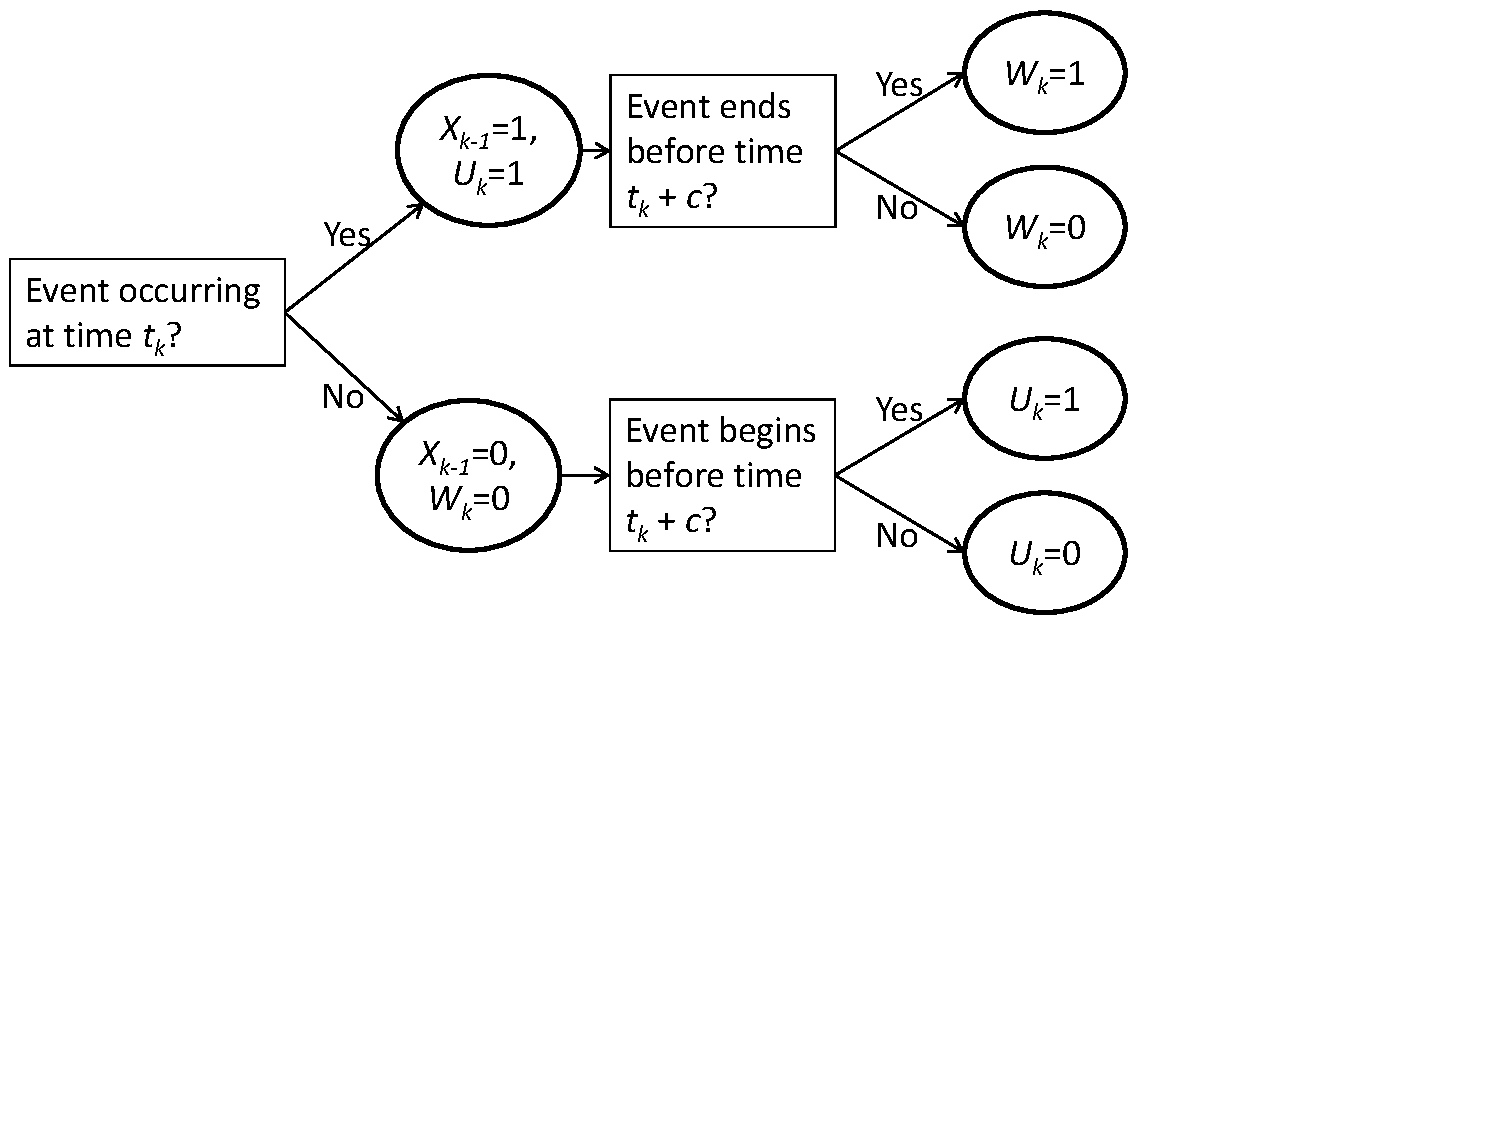
\includegraphics[clip=true, trim= 0 240 150 00, width=0.8\linewidth]{AIR_flowchart.pdf}
\caption{Procedure for combining MTS and interval recording}
\label{fig:questions}
\end{figure}  

The AIR procedure requires only marginally more effort on the part of the observer than an interval recording method used alone. 
One measure of effort is the level of sustained attention required on the part of the observer. Because the sustained attention needed for interval recording also entails the attention needed for momentary time sampling, the additional effort is minimal in this respect. 
Another measure of effort is the amount of data that must be recorded during the observation period. Because $W_k = 0$ is implied when $X_{k-1} = 0$ and $U_k = 1$ is implied when $X_{k-1} = 1$, AIR requires twice as much data as one of the single methods (rather than three times as much, might be supposed). 
Thus, for a fixed interval length, simultaneous use of all three methods entails at most twice as much effort as interval recording alone. 
Furthermore, using longer time-intervals with fewer intervals per observation period would mitigate the effort required.

Under the assumptions of the Alternating Poisson Process, the data generated by the AIR system can be modeled using a discrete-time Markov Chain, from which estimates of prevalence and incidence can be obtained. The Markov property of the Alternating Poisson Process implies that the joint distribution can be written as
\begin{multline}
\Pr\left(X_0=x_0,X_1=x_1,U_1 = u_1, W_1 = w_1,..., X_K=x_K, U_K = u_K, W_K = w_K \right) \\ = \Pr\left(X_0 = x_0\right) \prod_{k=1}^K \Pr\left(X_k = x_k, U_k = u_k, W_k = w_k | X_{k-1} = x_{k-1}\right). 
\end{multline}
Denote the transition probabilities $\Pr\left(X_k = b, U_k = c, W_k = d | X_{k-1} = a\right) = \pi_{a|bcd}$ and let $m_{a|bcd} = \sum_{k=1}^K I\left(X_{k-1} = a, X_k = b, U_k = c, W_k = d \right)$ for $a,b,c,d = 0,1$. Conditional on $X_0$, the log-likelihood of the observed AIR data is given by
\begin{equation}
\label{eq:AIR_loglik}
l_{AIR}\left(\phi,\zeta\right) = \sum_{a=0}^1 \sum_{b=0}^1 \sum_{c=0}^1 \sum_{d=0}^1 m_{a|bcd} \log \pi_{a|bcd}
\end{equation}
where
\begin{align*}
\pi_{0|000} &= \left[1 - p_0(d)\right]\exp\left(\frac{- \zeta c}{1 - \phi}\right) \\
\pi_{0|010} &= 1 - p_0(c + d) - \left[1 - p_0(d)\right]\exp\left(\frac{- \zeta c}{1 - \phi}\right) \\
\pi_{0|100} &= p_0(d)\exp\left(\frac{- \zeta c}{1 - \phi}\right) \\
\pi_{0|110} &= p_0(c + d) - p_0(d) \exp\left(\frac{- \zeta c}{1 - \phi}\right) \\
\pi_{1|010} &= 1 - p_1(c + d) - \left[1 - p_1(d)\right]\exp\left(\frac{- \zeta c}{\phi}\right) \\
\pi_{1|011} &= \left[1 - p_1(d)\right]\exp\left(\frac{- \zeta c}{\phi}\right) \\
\pi_{1|110} &= p_1(c + d) - p_1(d) \exp\left(\frac{- \zeta c}{\phi}\right) \\
\pi_{1|111} &= p_1(d)\exp\left(\frac{- \zeta c}{\phi}\right)
\end{align*}
and the remaining tansition probabilities are all equal to zero. 
See Appendix \ref{app:AIR_derivation} for the derivation of these quantities.

\section{Discussion}
\label{sec:discussion}

\bibliographystyle{apacite}
\bibliography{\bibfile}
 
\appendix

\section{Derivation of PIR model}
\label{app:PIR_derivation}

The joint distribution of PIR observations depends on the conditional probabilities $\psi_k = \Pr\left[ Z(t_k) = 1 \left| U_1,...,U_{k-1}\right.\right]$. 
This appendix provides a derivation of Expression (\ref{eq:psi_k}) in terms of the parameters of the Alternating Poisson Process. The derivation will make use of the following lemma.

\begin{lemma}
\label{lemma1}
The conditional probabilities of $Z(t_k) = 1, U_{k-1} = 1$ given $Z(t_{k-1})$ are:
\begin{align*}
\Pr\left(Z(t_k) = 1, U_{k-1} = 1 \left| Z(t_{k-1}) = 1 \right.\right) &= p_1(c + d) \\
\Pr\left(Z(t_k) = 1, U_{k-1} = 1 \left| Z(t_{k-1}) = 0 \right.\right) &= p_0(c + d) - p_0(d) \exp\left(\frac{- \zeta c}{1 - \phi}\right).
\end{align*}
\end{lemma}

\begin{proof}
Observe that \[
\Pr\left(Z(t_k) = 1, U_{k-1} = 1 \left| Z(t_{k-1}) = 1 \right.\right) = \Pr\left(Z(t_k) = 1 \left| Z(t_{k-1}) = 1 \right.\right) = p_1(c + d) \]
and \begin{align*}
\Pr &\left(Z(t_k) = 1, U_{k-1} = 1 \left| Z(t_{k-1}) = 0 \right.\right) \\
& \qquad \qquad = \int_0^c\frac{p_1(c - t) \zeta}{(1 - \phi)}\exp\left(\frac{-\zeta t}{1 - \phi}\right) dt \\
& \qquad \qquad  = \phi \left[ 1 - \exp\left(\frac{- \zeta (c + d)}{\phi(1 - \phi)}\right) - \exp\left(\frac{- \zeta c}{1 - \phi}\right) + \exp\left(\frac{- \zeta (\phi c + d)}{\phi(1 - \phi)}\right)\right] \\
& \qquad \qquad = p_0(c + d) - p_0(d) \exp\left(\frac{- \zeta c}{1 - \phi}\right).
\end{align*}
\end{proof}

Turning to the derivation of $\psi_k$, begin by noting that $U_{k-1} = 0$ implies that $Z(t_k + c) = 0$. 
It follows from the Markov property that 
\begin{multline*}
\Pr\left(Z(t_k) = 1 \left| U_1 = u_1,...,U_{k-2} = u_{k-2}, U_{k-1} = 0 \right.\right) \\ 
= \Pr\left(Z(t_k) = 1 \left| Z(t_{k-1} + c) = 0 \right.\right) = p_0(d).
\end{multline*}
Next, Lemma \ref{lemma1} implies that \begin{multline*}
\Pr\left(Z(t_k) = 1, U_{k-1} = 1 \left| U_1,...,U_{k-2} \right.\right) \\
= \psi_{k-1} p_1(c + d) + (1 - \psi_{k-1}) \left[p_0(c + d) - p_0(d) \exp\left(\frac{- \zeta c}{1 - \phi}\right)\right].
\end{multline*}
It therefore follows that 
\begin{multline*}
\Pr\left(Z(t_k) = 1 \left| U_1 = u_1,...,U_{k-2} = u_{k-2}, U_{k-1} = 1 \right.\right) \\
= \frac{\psi_{k-1} p_1(c + d) + (1 - \psi_{k-1}) \left[p_0(c + d) - p_0(d) \exp\left(\frac{- \zeta c}{1 - \phi}\right)\right]}{1 - (1 - \psi_{k-1})\exp\left( \frac{-\zeta c}{1 - \phi}\right)}.
\end{multline*}
Thus, $\psi_k$ can be written as a function of $\psi_{k-1}$ and $u_{k-1}$, as given in (\ref{eq:psi_k}).

\section{Derivation of AIR model}
\label{app:AIR_derivation}

This appendix provides a derivation of the transition probabilities for the AIR model in terms of the parameters of the Alternating Poisson Process. Begin by noting that, by the definitions of the recording procedures, $X_{k-1} = 0$ implies that $W_k = 0$ and $X_{k-1} = 1$ implies that $U_k = 1$. It follows that $\pi_{0|bc1} = 0$ for $b,c = 0,1$ and $\pi_{1|b0d} = 0$ for $b,d=0,1$. Derivation of the other transition probabilities will make use of the following lemma. (The proof follow the same logic as in Lemma \ref{lemma1}, and is therefore omitted.)

\begin{lemma}
\label{lemma2}
The conditional probability of $Z(t_k) = 1, W_{k-1} = 0$ given that $Z(t_{k-1}) = 1$ is
\[
\Pr\left(Z(t_k) = 1, W_{k-1} = 0 \left| Z(t_{k-1}) = 1 \right.\right) = p_1(c + d) - p_1(d) \exp\left(\frac{- \zeta c}{\phi}\right). \]
\end{lemma}

Turning to the eight remaining transition probabilities, note that
\begin{align*}
\pi_{0|100} &= \Pr\left(X_k = 1, U_k = 0 | X_{k-1} = 0\right) \\
&= \Pr\left(X_k = 1 | Z(t_k + c) = 0\right) \Pr\left(U_k = 0 | X_{k-1} = 0\right) \\
&= p_0(d)\exp\left(\frac{- \zeta c}{1 - \phi}\right).
\end{align*}
Similarly,
\begin{align*}
\pi_{0|000} &= \Pr\left(X_k = 0, U_k = 0 | X_{k-1} = 0\right) = \left[1 - p_0(d)\right]\exp\left(\frac{- \zeta c}{1 - \phi}\right) \\
\pi_{1|111} &= \Pr\left(X_k = 1, W_k = 1 | X_{k-1} = 1\right) = p_1(d)\exp\left(\frac{- \zeta c}{\phi}\right) \\
\pi_{1|011} &= \Pr\left(X_k = 0, W_k = 1 | X_{k-1} = 1\right) = \left[1 - p_1(d)\right]\exp\left(\frac{- \zeta c}{\phi}\right).
\end{align*}
Next, it follows from Lemmas \ref{lemma1} and \ref{lemma2} that
\begin{align*}
\pi_{0|110} &= \Pr\left(X_k = 1, U_k = 1 | X_{k-1} = 0\right) = p_0(c + d) - p_0(d) \exp\left(\frac{- \zeta c}{1 - \phi}\right) \\
\pi_{1|110} &= \Pr\left(X_k = 1, W_k = 0 | X_{k-1} = 1\right) = p_1(c + d) - p_1(d) \exp\left(\frac{- \zeta c}{\phi}\right).
\end{align*}
The two remaining transition probabilities can be obtained by subtraction:
\begin{align*}
\pi_{0|010} &= 1 - \pi_{0|000} - \pi_{0|100} - \pi_{0|110} = 1 - p_0(c + d) - \left[1 - p_0(d)\right]\exp\left(\frac{- \zeta c}{1 - \phi}\right) \\
\pi_{1|010} &= 1 - \pi_{1|011} - \pi_{1|110} - \pi_{1|111} = 1 - p_1(c + d) - \left[1 - p_1(d)\right]\exp\left(\frac{- \zeta c}{\phi}\right).
\end{align*}
\end{document}
